\subsection{Residual Channel Attention Network (RCAN\cite{RCAN})}\label{rcan}

In SR task in order to reconstruct an SR image \textit{high-frequency information} are extremely important, therefore \textbf{attention} mechanism are deployed in order to do so.

As usual the depth is also important hence the use of residuals which allow to have a deeper network avoiding exploding/vanishing gradient.

\subsubsection{Architecture}
\begin{figure}
    \centering
    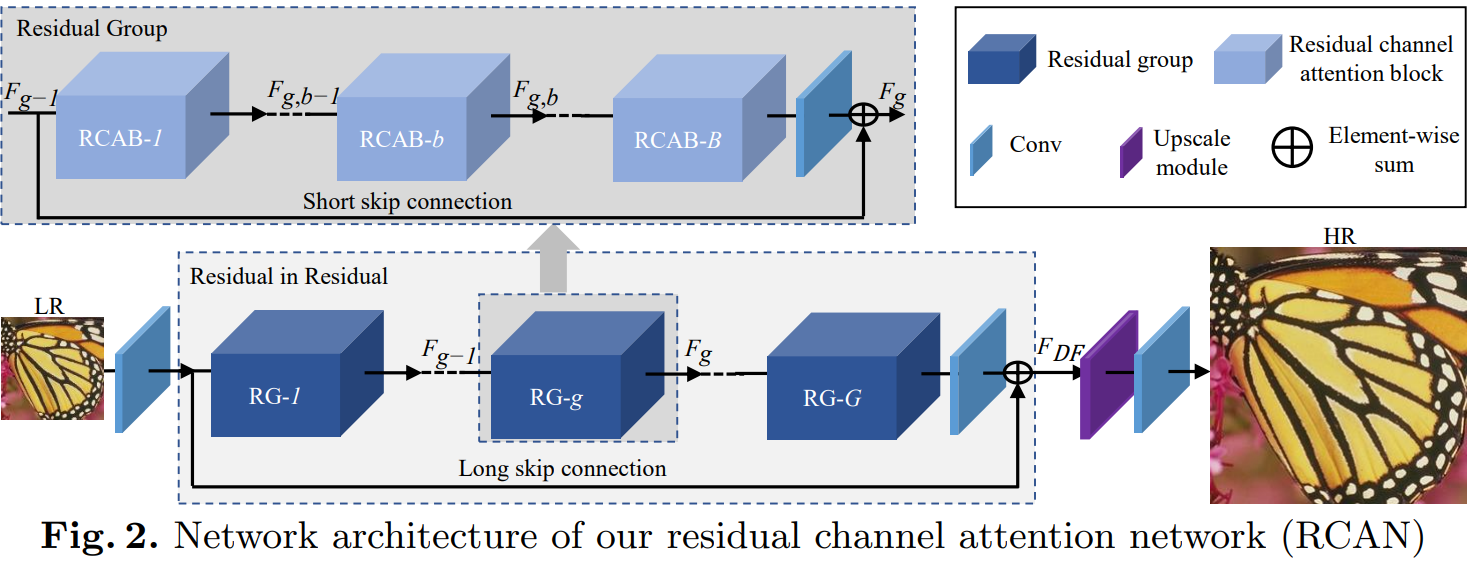
\includegraphics[width=\textwidth, keepaspectratio]{rcan-model.png}
    \caption{RCAN architecture.}\label{rcan:model}
\end{figure}
\begin{figure}
    \centering
    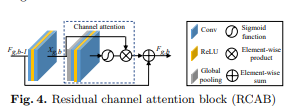
\includegraphics[width=\textwidth, keepaspectratio]{rcan-rcab.png}
    \caption{Residual channel attention block.}\label{rcan:rcab}
\end{figure}


\Cref{rcan:model} highlights:
\begin{itemize}
    \item \textbf{shallow extractor} for extracting low level features
    \item deep features extractor using \textbf{Residual in Residual (RIR)}: the main module is the residual groups (\textbf{RG}) created using a sequence of \textbf{RCAB}[\Cref{rcan:rcab}] where short skip connection are present which with the long skip connection allow to ease the training and reduce the amount of low-frequency information in the network because directly extracted from the LR image.
    There are \textbf{G} residual groups composed by \textbf{B} \textit{residual channel attention blocks}.
    \item \textbf{upscaling module} using \textit{transposed convolution}, \textit{nearest neighbor and convolution}, \textit{subpixel convolution}.
    \item \textbf{reconstruction} using a single convolution.
\end{itemize}

\paragraph{Channel attention}
The \textbf{Channel attention} has to capture high-frequency information inside the features extracted by convolutions; in order to do so a global statistics of the features is computed using global average pooling channel-wise which are further processed in order to create a mask using a sigmoid activation which allow to create a non mutual-exclusive mask and non-linear information which allow to increase the expressing power of the network.
\begin{figure}
    \centering
    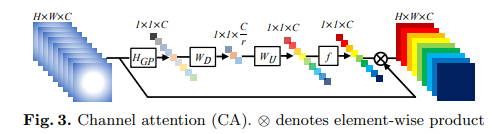
\includegraphics[width=\textwidth, keepaspectratio]{rcan-channel-attention-module.png}
    \caption{Channel attention used in RCAB.}\label{rcan:channelattention}
\end{figure}

\subsubsection{Results}

\paragraph{Ablation studies on LSC, SSC and CA}
From \Cref{rcan:ablationstudies} it's possible to see that short-skip connections (SSC) and long-skip connections (LSC) are extremely important but in order to improve the final results channel attention is necessary.
\begin{figure}[H]
    \centering
    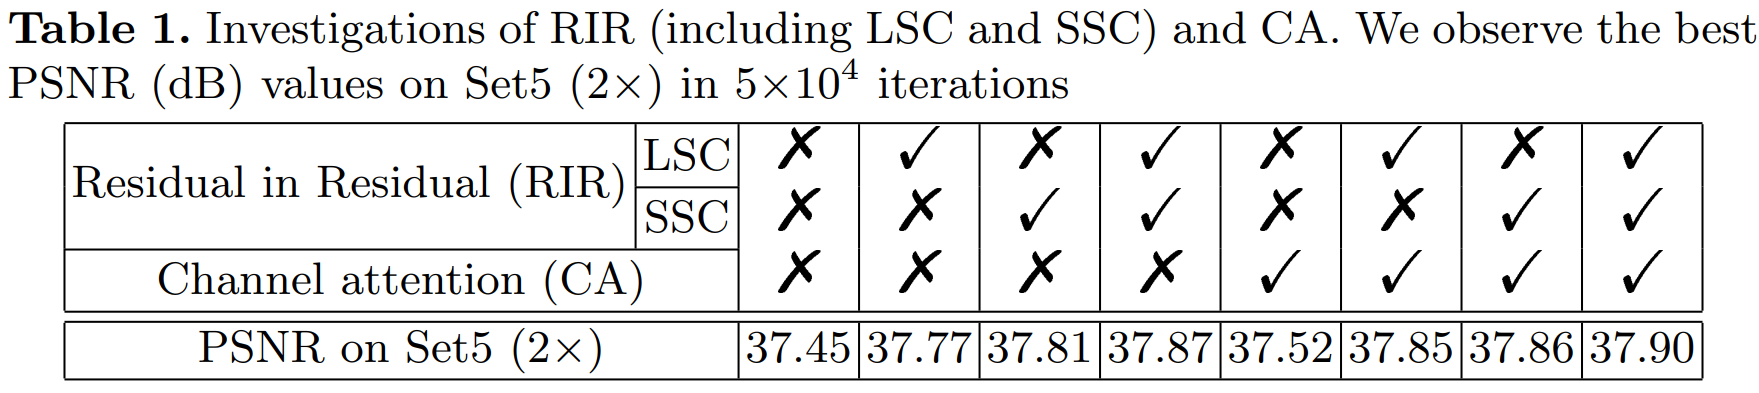
\includegraphics[width=\textwidth, keepaspectratio]{rcan-ablation-studies.png}
    \caption{Ablation studies done on RCAN.}\label{rcan:ablationstudies}
\end{figure}

\paragraph{Quantitative and qualittive results}
\subparagraph{Using Bicubic as degradation model}
Thanks to the depth and channel attention RCAN is able to reconstruct the original HR image without artifact or blurring.
\begin{figure}[H]
    \centering
    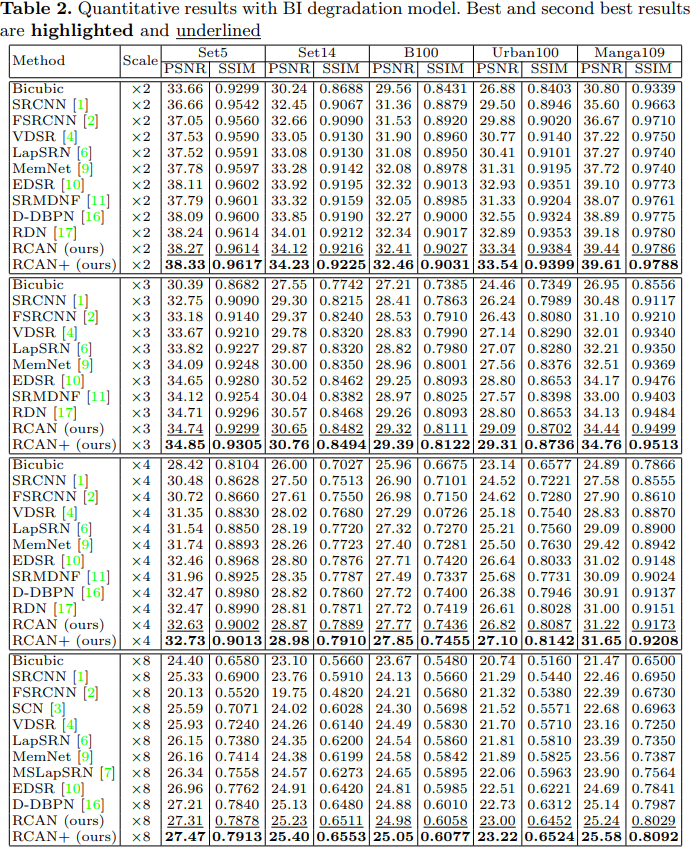
\includegraphics[width=\textwidth, keepaspectratio]{rcan-quantitative.png}
    \caption{Quantitative results of RCAN.}
\end{figure}
\begin{figure}[H]
    \centering
    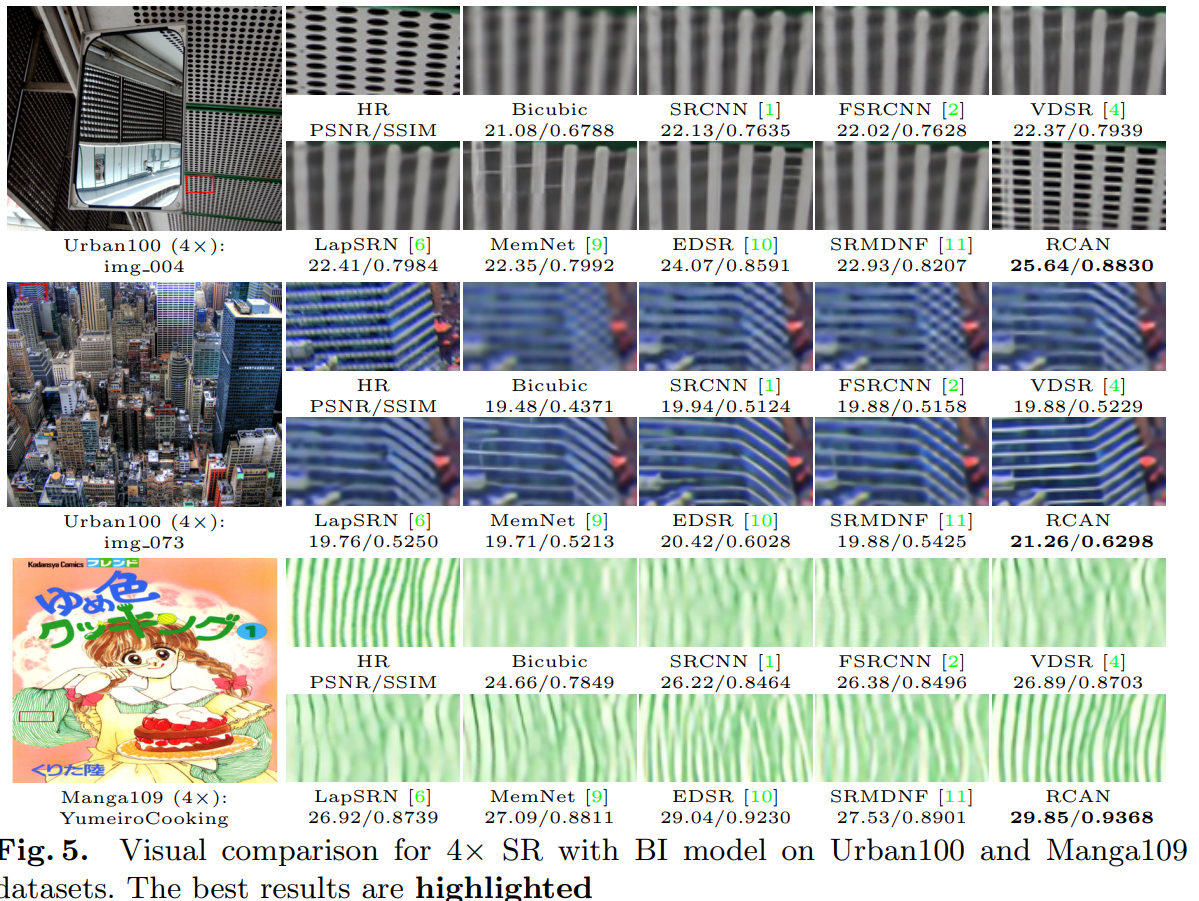
\includegraphics[width=\textwidth, keepaspectratio]{rcan-qualitative.png}
    \caption{Qualitative results of RCAN.}
\end{figure}

\subparagraph{Using Blur-Down degradation model}
RCAN performs better than any state-of-the-art.
\begin{figure}[H]
    \centering
    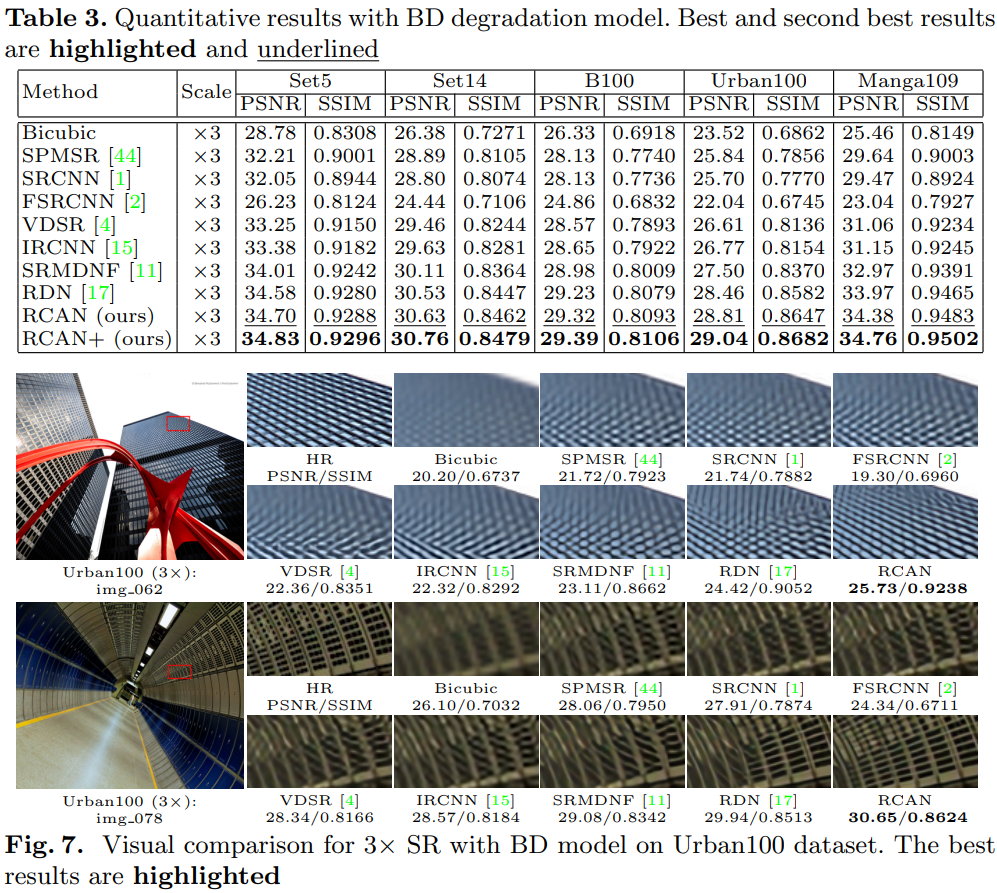
\includegraphics[width=\textwidth, keepaspectratio]{rcan-qq-bd-results.png}
    \caption{Quantitative and qualitative results of RCAN using blur as degradation.}
\end{figure}

\subparagraph{With object recognition task}
Using RCAN for upscaling an 56x56 image to 256x256 achieves the lowest top-1 and top-5 errors in object detection.
\begin{figure}[H]
    \centering
    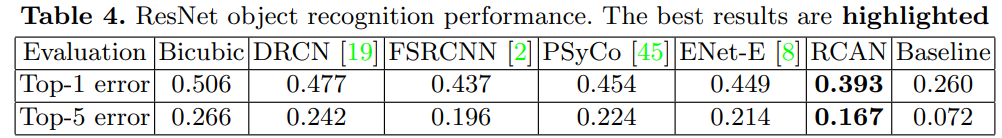
\includegraphics[width=\textwidth, keepaspectratio]{rcan-obj-rec-results.png}
    \caption{RCAN used at the beginning of a pipeline (upsamples an image to 224x244) for object recognition}
\end{figure}

\paragraph{Performance versus Parameters}
RCAN achieve the best performance with not so many parameters.
\begin{figure}[H]
    \centering
    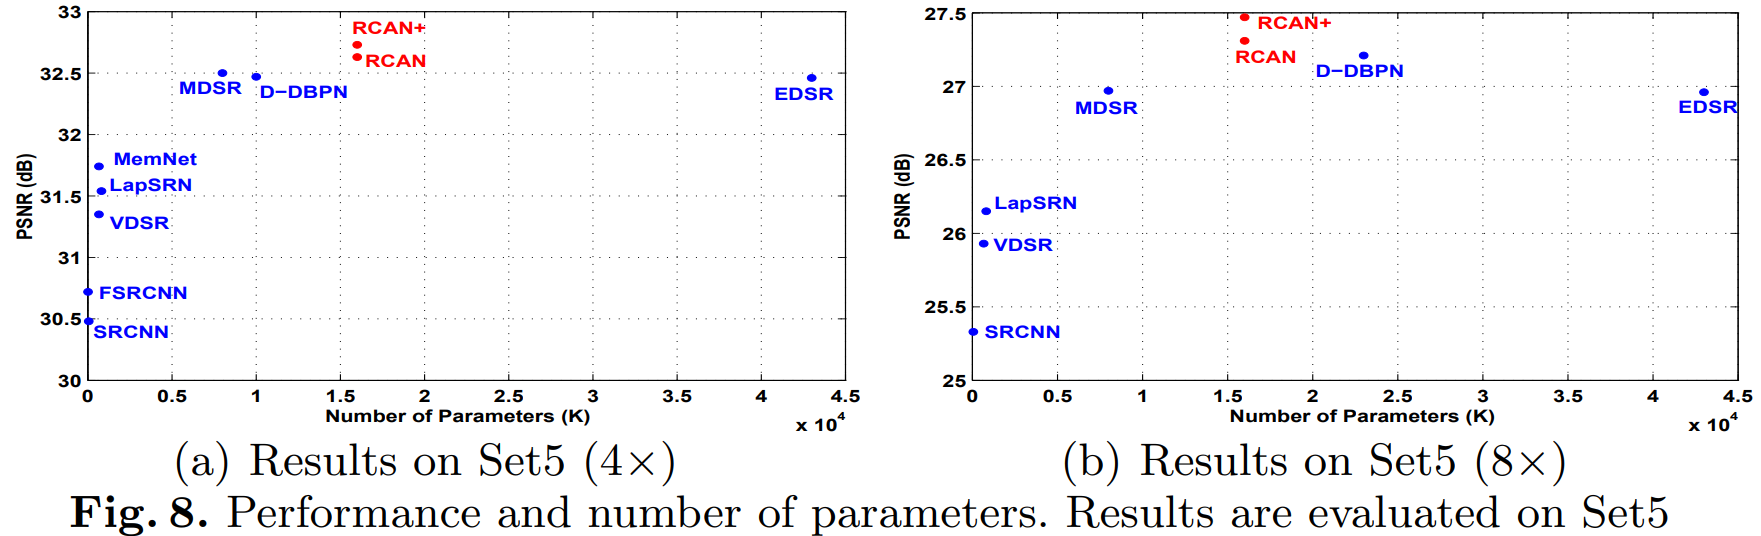
\includegraphics[width=\textwidth, keepaspectratio]{rcan-performance-params.png}
    \caption{Comparison of parameters and performance of state-of-the-art SR network.}
\end{figure}